\documentclass[tikz,border=12pt]{standalone}
\usepackage[T1]{fontenc}
\usepackage{mathpazo}
\usepackage{amsmath,amssymb}
\usetikzlibrary{arrows.meta, positioning, calc, fit}

\definecolor{stblue}{HTML}{7B97AD}
\definecolor{rwgold}{HTML}{B8995E}
\definecolor{sage}{HTML}{7A9A7E}
\definecolor{dkbrown}{HTML}{3D3530}
\definecolor{wmgray}{HTML}{7B7067}
\definecolor{cream}{HTML}{F9F6F0}
\definecolor{border}{HTML}{D4C9B8}
\definecolor{terracotta}{HTML}{C47A6A}

\begin{document}
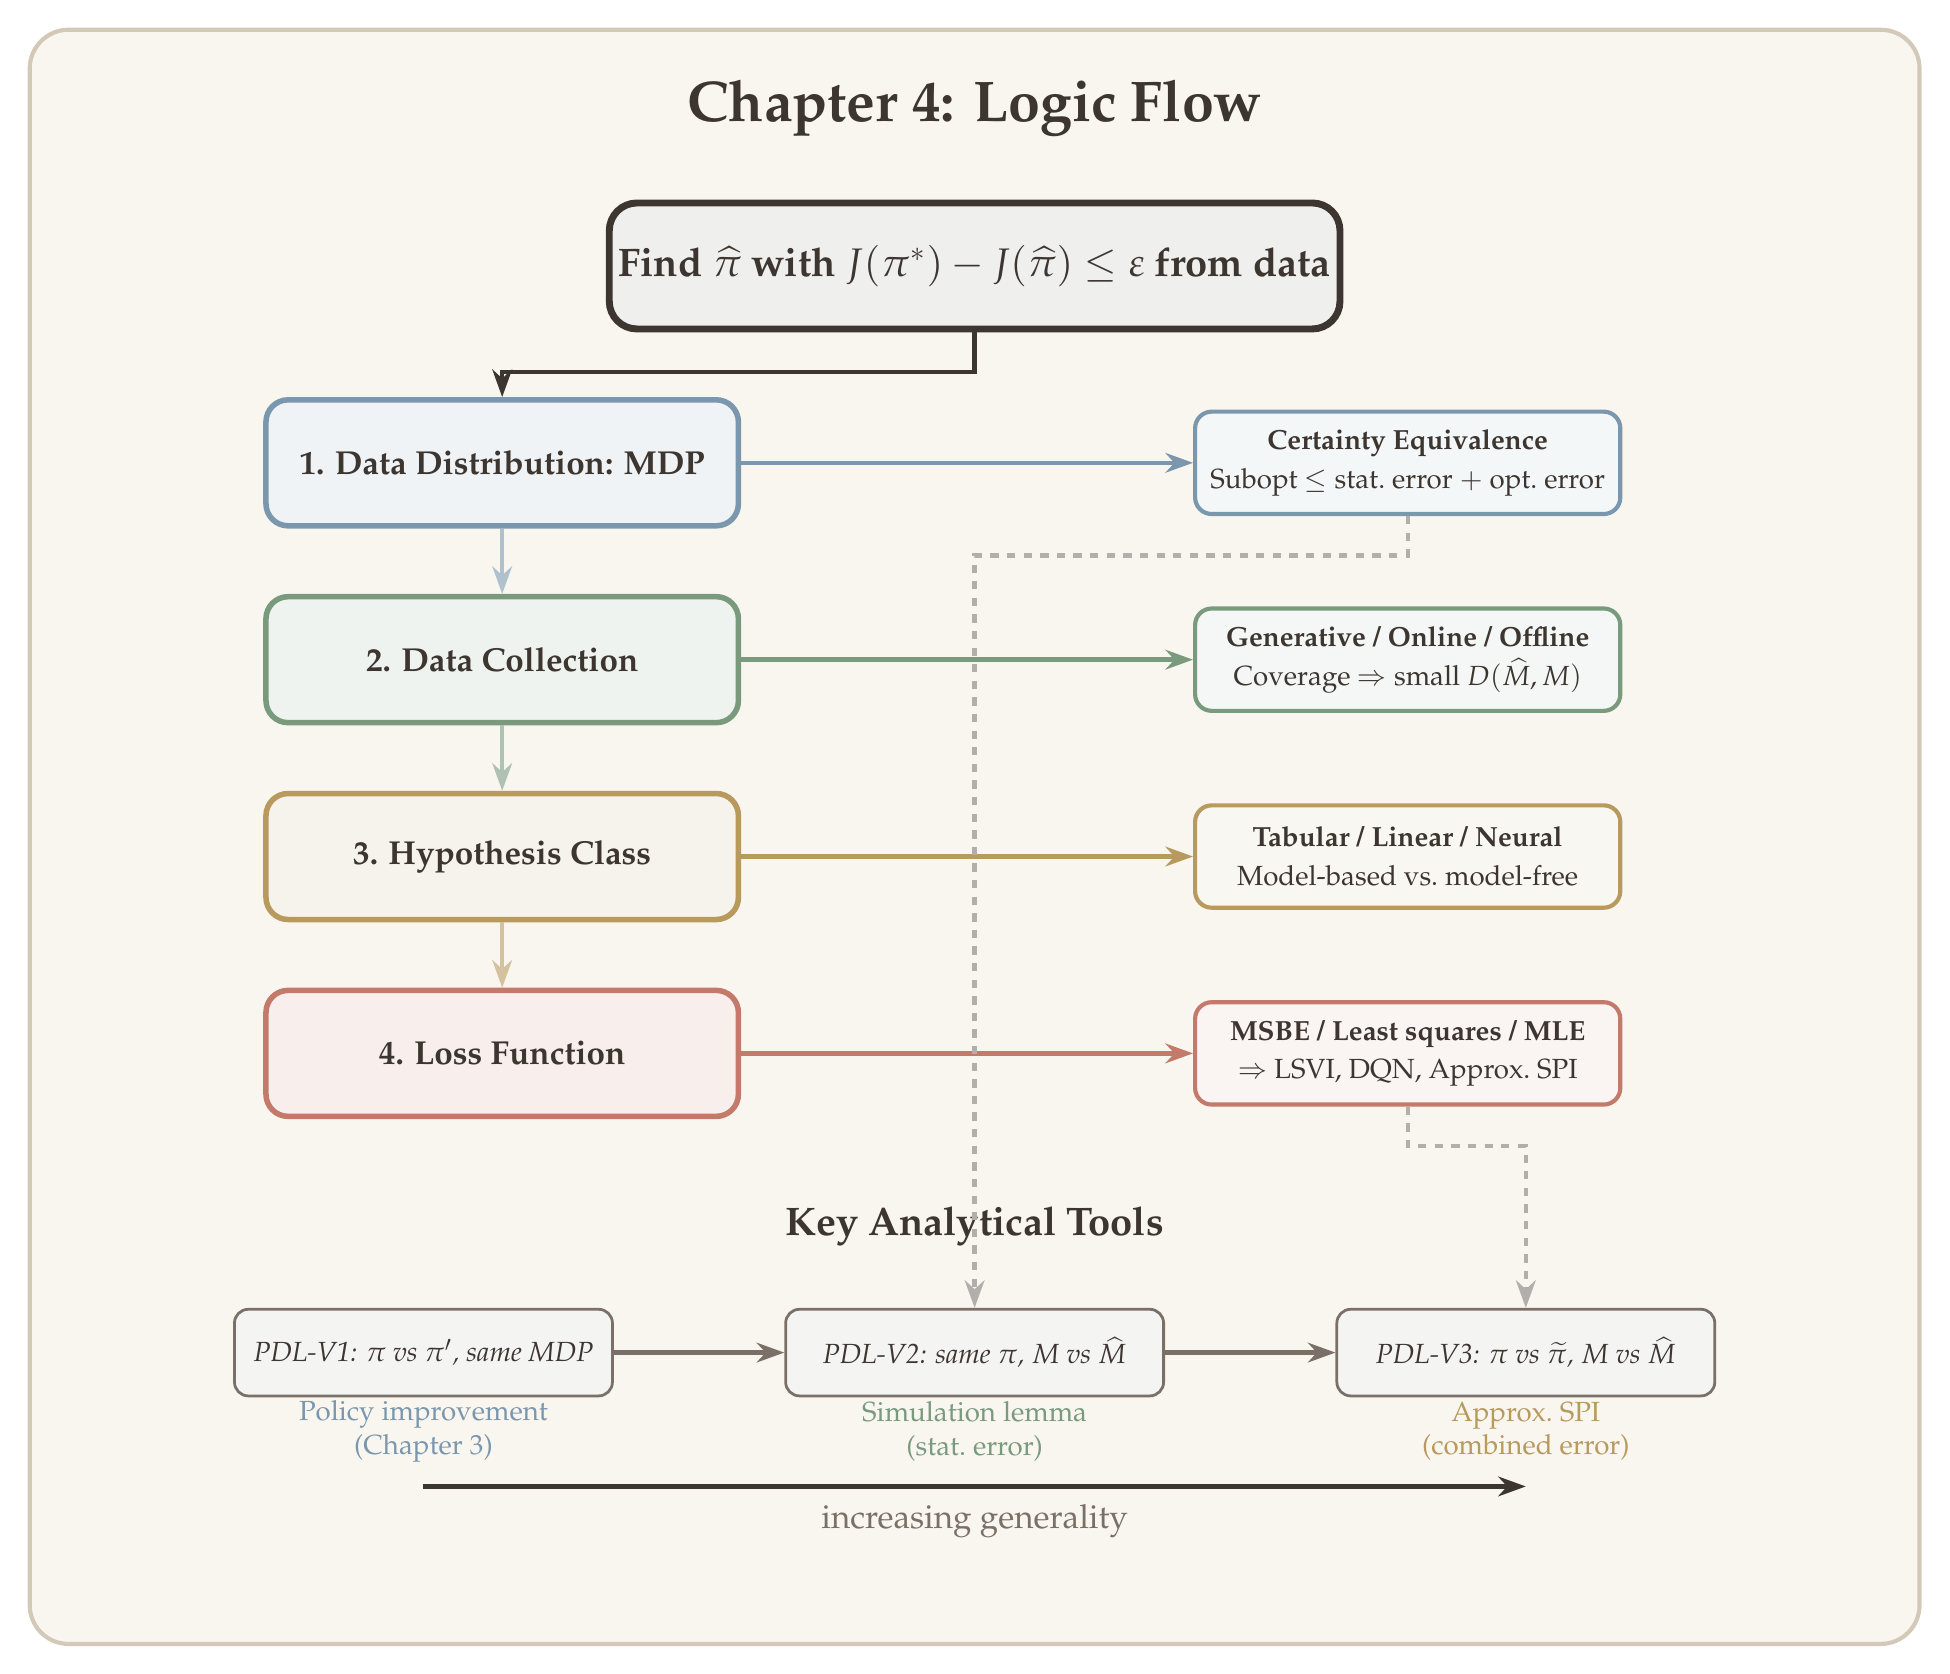
\begin{tikzpicture}[
  >={Stealth[length=3.5mm, width=2.5mm]},
  element/.style={draw=#1, line width=2pt, fill=#1!12, rounded corners=8pt,
    minimum width=60mm, minimum height=16mm, font=\large\bfseries, text=dkbrown,
    align=center, inner sep=5pt},
  result/.style={draw=#1, line width=1.5pt, fill=#1!8, rounded corners=6pt,
    minimum width=54mm, minimum height=13mm, font=\normalsize, text=dkbrown,
    align=center, inner sep=5pt},
  tool/.style={draw=wmgray, line width=1pt, fill=wmgray!8, rounded corners=5pt,
    minimum width=48mm, minimum height=11mm, font=\normalsize\itshape, text=dkbrown,
    align=center, inner sep=4pt},
  arr/.style={->, line width=1.6pt, dkbrown},
]

% Background
\fill[cream, rounded corners=14pt] (-1.5,-14.5) rectangle (22.5,6.0);
\draw[border, rounded corners=14pt, line width=1.5pt] (-1.5,-14.5) rectangle (22.5,6.0);

% Title
\node[font=\huge\bfseries, text=dkbrown] at (10.5,5.0)
  {Chapter 4: Logic Flow};

% =============================================
% Top: Central Question
% =============================================
\node[draw=dkbrown, line width=2.5pt, fill=dkbrown!8, rounded corners=10pt,
  minimum width=80mm, minimum height=16mm, font=\Large\bfseries, text=dkbrown,
  align=center] (question) at (10.5,3.0)
  {Find $\widehat{\pi}$ with $J(\pi^*) - J(\widehat{\pi}) \leq \varepsilon$ from data};

% =============================================
% Four Elements (left column)
% =============================================
\node[element=stblue] (e1) at (4.5,0.5)
  {1. Data Distribution: MDP};

\node[element=sage] (e2) at (4.5,-2.0)
  {2. Data Collection};

\node[element=rwgold] (e3) at (4.5,-4.5)
  {3. Hypothesis Class};

\node[element=terracotta] (e4) at (4.5,-7.0)
  {4. Loss Function};

\draw[arr] (question.south) -- ++(0,-0.5) -| (e1.north);
\draw[arr, stblue!60] (e1.south) -- (e2.north);
\draw[arr, sage!60] (e2.south) -- (e3.north);
\draw[arr, rwgold!60] (e3.south) -- (e4.north);

% =============================================
% Results for each element (right column)
% =============================================
% E1 -> Certainty equivalence
\node[result=stblue] (r1) at (16.0,0.5)
  {\textbf{Certainty Equivalence}\\[2pt]
   Subopt $\leq$ stat.\ error $+$ opt.\ error};

\draw[arr, stblue] (e1.east) -- (r1.west);

% E2 -> Three settings, coverage requirement
\node[result=sage] (r2) at (16.0,-2.0)
  {\textbf{Generative / Online / Offline}\\[2pt]
   Coverage $\Rightarrow$ small $D(\widehat{M}, M)$};

\draw[arr, sage] (e2.east) -- (r2.west);

% E3 -> Function approximation
\node[result=rwgold] (r3) at (16.0,-4.5)
  {\textbf{Tabular / Linear / Neural}\\[2pt]
   Model-based vs.\ model-free};

\draw[arr, rwgold] (e3.east) -- (r3.west);

% E4 -> Loss functions and algorithms
\node[result=terracotta] (r4) at (16.0,-7.0)
  {\textbf{MSBE / Least squares / MLE}\\[2pt]
   $\Rightarrow$ LSVI, DQN, Approx.\ SPI};

\draw[arr, terracotta] (e4.east) -- (r4.west);

% =============================================
% Bottom: Key tools
% =============================================
\node[font=\Large\bfseries, text=dkbrown] at (10.5,-9.2)
  {Key Analytical Tools};

\node[tool] (pdl1) at (3.5,-10.8)
  {PDL-V1: $\pi$ vs $\pi'$, same MDP};
\node[tool] (pdl2) at (10.5,-10.8)
  {PDL-V2: same $\pi$, $M$ vs $\widehat{M}$};
\node[tool] (pdl3) at (17.5,-10.8)
  {PDL-V3: $\pi$ vs $\widetilde{\pi}$, $M$ vs $\widehat{M}$};

\draw[arr, wmgray] (pdl1.east) -- (pdl2.west);
\draw[arr, wmgray] (pdl2.east) -- (pdl3.west);

% Labels below
\node[font=\normalsize, text=stblue, align=center] at (3.5,-11.8) {Policy improvement\\(Chapter 3)};
\node[font=\normalsize, text=sage, align=center] at (10.5,-11.8) {Simulation lemma\\(stat.\ error)};
\node[font=\normalsize, text=rwgold, align=center] at (17.5,-11.8) {Approx.\ SPI\\(combined error)};

% Link from results down to tools
\draw[arr, dkbrown!40, dashed] (r1.south) -- ++(0,-0.5) -| (pdl2.north);
\draw[arr, dkbrown!40, dashed] (r4.south) -- ++(0,-0.5) -| (pdl3.north);

% =============================================
% Arrow showing generalization
% =============================================
\draw[dkbrown, line width=2pt, ->] (3.5,-12.5) -- (17.5,-12.5);
\node[font=\large, text=wmgray, anchor=north] at (10.5,-12.6)
  {increasing generality};

\end{tikzpicture}
\end{document}
